\chapter{The record, 6--10 November 2026}\label{ch:november}

This chapter adds the studies committed between the 6 November survey and
10 November (commit \texttt{13df75511}). None of their directories was cited
in the chapters above. Every number is copied from the named artefact; the
plotted values, with file and line, are in
\art{figures/data-november.json}, and \art{figures/make_fig_november.py}
draws the figures. Almost every source marks its numbers
\texttt{[pcc:unverified]}, and none has a validation file or a leaderboard
row. Read them as producer records, not admitted results.

Four things changed:
\begin{itemize}
\item \emph{The generic track on the Curve25519 miniatures moved closer to
  rho, and then stopped.} An arm that walks from the target reached
  $1.37$--$1.40\times$ rho-neg at $k=28$--$32$. Without the per-collision
  recompute it reached $1.22$--$1.26\times$ at $k=20$--$24$. These arms are
  one unknown away from rho and are not decomposition index calculus
  (\S\ref{sec:nov-generic}).
\item \emph{Two accounting changes, owner-adopted or settled, moved the
  references.} Table inserts are priced by default from 8 November. The
  prime medium-tier rho sits at $1.067\times$ its floor, so prime gaps
  normalised to toy rho were understated by about $1.27\times$
  (\S\ref{sec:nov-reference}). Both are \cls{accounting} changes.
\item \emph{The $k=4$ characteristic-two ladder reached $m=18$.} IC is
  $0.45\times$ rho's theoretical cost there, on one target with its rho run
  unfinished. The crossover is indicated, not established
  (\S\ref{sec:nov-k4}).
\item \emph{Every prime-field lead tested in the window closed or stayed
  open without a lever} (\S\ref{sec:nov-prime}). One example is minors
  guess-and-determine, whose gap to rho grows from $4.37\times$ at 20 bits
  to $1552\times$ at 40 bits.
\end{itemize}

\section{The generic track on Curve25519 miniatures}\label{sec:nov-generic}

Section~\ref{sec:gf-bsgs} left the autolab incumbent at about $1.8$--$1.9\times$
rho-neg, at the $F=2$ collision floor. The November studies changed the
\emph{shape} of the arm rather than tuning it.
\begin{itemize}
\item \emph{One seed ($F=1$).} A one-seed walk table beat the $F=2$
  \texttt{wwalk} incumbent. The ratio was $0.809$ $[0.776,0.842]$ at $k=20$ and
  $0.855$ $[0.814,0.898]$ at $k=24$, $w=0$. Against rho-neg the arm
  \texttt{f1-x07} stays at $1.496$--$1.595\times$ over $k=20$--$32$
  (\art{research/curve25519_f1_walk_20261107/README.md},
  \art{research/curve25519_tw_scaling_20261108/README.md}).
\item \emph{Target in the walk.} Starting the walk from the target with chained jumps
  (\texttt{twcj}) beat \texttt{f1-x07} by $0.909$ $[0.885,0.934]$ at $k=20$
  and $0.888$ $[0.846,0.932]$ at $k=24$
  (\art{research/curve25519_f1_targetwalk_20261108/README.md}).
  \begin{itemize}
  \item Four jumps were worse than sixteen: $1.220$ $[1.186,1.256]$ and
    $1.268$ $[1.193,1.348]$ at $k=20,24$
    (\art{research/curve25519_tw_jumps_20261108/README.md}).
  \item Thirty-two and sixty-four jumps were nulls against sixteen:
    $0.997$ $[0.954,1.041]$ at $k=28$ and $0.985$ $[0.930,1.044]$ at $k=32$.
  \item At $k=32$, \texttt{twcj-j16} costs $1.366$ $[1.267,1.473]\times$
    rho-neg. Its walk is $1.368\sqrt r$, 3\% above the second-collision floor
    of $1.329\sqrt r$. Rho-neg's search is $0.999\sqrt r$, 13\% above its
    first-collision floor of $0.886\sqrt r$
    (\art{research/curve25519_tw_scaling_20261108/README.md}).
  \end{itemize}
\item \emph{Dropping the per-collision recompute} (engine item A,
  \texttt{cv\,=\,0}) cut a further $0.879$ $[0.876,0.881]$ at $k=20$ and
  $0.950$ $[0.948,0.951]$ at $k=24$. That leaves $1.217$ $[1.166,1.271]$ and
  $1.259$ $[1.187,1.336]\times$ rho-neg. A chained set-up for rho-neg itself
  (item B) was rejected as a reference: it is $1.532\times$ and
  $2.738\times$ dearer (\art{research/curve25519_engine_items_20261110/README.md}).
\item \emph{Autolab.} Rounds 36 and 37 (10 November) improved $k=24$
  ($0.924$ $[0.857,0.996]$) and $k=32$ ($0.915$ $[0.864,0.969]$). The other
  sizes were null, and the distance stays near $1.8\times$
  (\art{research/curve25519_autolab_20261104/round-036/},
  \art{round-037/}). The five-curve SNC panel puts \texttt{tw2cj-lazy} at
  $1.61$--$1.78\times$ rho against the incumbent's $1.72$--$1.94\times$
  (\art{research/curve25519_autolab_20261104/snc-panel/README.md}).
\end{itemize}

\paragraph{What these arms are.} Every source makes the same scope remark.
Setting the one unknown seed to $G$ turns the arm into rho with a stored
walk. These are therefore boundary methods in the sense of
\S\ref{sec:gf-bsgs}, not decomposition index calculus, and the
$F=1$ collision floor of $1.5\times$ does not bind them. Their remaining
distance is rho's own floor ratio: second collision against first.

\begin{figure}[t]
\centering
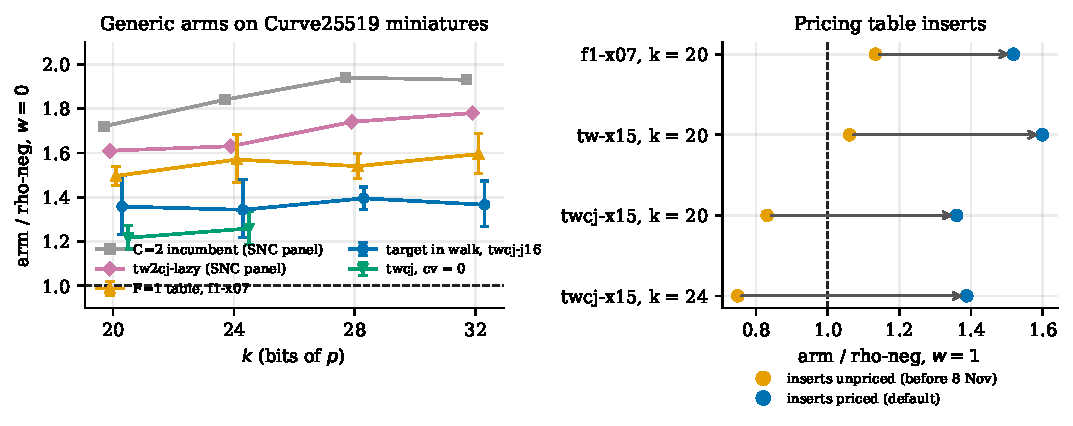
\includegraphics[width=\linewidth]{figures/fig-nov-generic.pdf}
\caption[]{Left: generic arms on the Curve25519-family miniatures, arm over
rho-neg at $w=0$ (95\% intervals where the source gives them; SNC rows are
five-curve means). Right: walk-table arms over rho-neg at $w=1$, before and
after table inserts were priced (\S\ref{sec:nov-reference}). Sources:
\art{research/curve25519_tw_jumps_20261108/},
\art{research/curve25519_tw_scaling_20261108/},
\art{research/curve25519_f1_walk_20261107/},
\art{research/curve25519_engine_items_20261110/},
\art{research/curve25519_autolab_20261104/snc-panel/},
\art{research/ecbench_table_work_pricing_20261108/}; values in
\art{figures/data-november.json}.}
\label{fig:nov-generic}
\end{figure}

\paragraph{Algebraic and structural routes on the same curves.} None closes
the gap.
\begin{itemize}
\item \emph{Oracle search} (\art{research/curve25519_algebraic_oracle_search_20261107/README.md}).
  The best non-generic oracle is $821\times$ behind rho-neg at $w=0.1$. The
  screen's best row was generic: its $S_3$ root-find is $x(R\pm P_1)$ on
  2{,}000 of 2{,}000 instances, so that row is baby-step giant-step with an
  unknown base, $251\times$ behind.
\item \emph{Structure audit} (\art{research/curve25519_structure_vs_rho_20261107/README.md}).
  The best lever costs at least $16.7\times$ rho-neg at $w=0.1$. Here
  $\mathrm{End}(E)=\ZZ[\pi]$, so the least non-scalar endomorphism has
  degree 772{,}948 ($2134\sqrt r$).
\item \emph{Exponent study} (\art{research/curve25519_exponent_study_20261108/README.md}).
  At $m=2$ the F4 cost grows as $|V|^s$ with $s=2.77$ $[2.31,3.23]$ at $k=20$.
  At $m=3,4$ the series was cut off by the 3.5\,GB / 1{,}200\,s limits, so
  the preregistered verdict is ``undetermined''.
\end{itemize}

\section{The references moved}\label{sec:nov-reference}

\paragraph{Table inserts are priced (\cls{accounting}).} Since 8 November
the \S5a band prices the per-step inserts of table oracles by default
(\art{research/ecbench_table_work_pricing_20261108/README.md}). With inserts
priced, every walk-table arm is above rho-neg at every weight. For example,
\texttt{twcj-x15} at $w=1$ moves from $0.831$ to $1.360$ at $k=20$ and from
$0.749$ to $1.388$ at $k=24$ (Figure~\ref{fig:nov-generic}, right). Pricing
one side and not the other moves a $w=1$ ratio by $0.4$ to $0.6$. Band
readings made before that date carry the label ``pre-2026-11-08 reading'',
and the priced ratios remain a lower bound on the walk arms' distance.

\paragraph{The prime medium-tier rho (\cls{accounting}).} Three studies settle
it (\art{research/prime_medium_tier_rho_20261107/},
\art{research/prime_medium_rho_p4_confirm_20261108/},
\art{research/prime_medium_rho_cpc_20261109/}). The third passed every gate:
$M=1.067$ $[0.999,1.134]$ times the floor and $\alpha=0.506$
$[0.483,0.529]$, over 432 \texttt{rho.negation} runs at
$\log_2 r=32.4$--$49.0$, verdict \texttt{setup\_excess}. Toy-tier prime rho
sits at about $1.38\times$ its floor. A prime IC gap normalised to toy rho
is therefore understated by about $1.27\times$. Gaps against a same-session
matched rho are unchanged.

\paragraph{The collision floor at $p_{36}$.} The matched \texttt{rho.negation}
costs $1.024$ $[0.961,1.091]$ times $\sqrt{\pi r/4}$, so the reference is
unbiased at this size (\art{research/ic_rho_floor_20261109/README.md}).
The earlier $1.32\times$ reading of \texttt{res1eq} was a small-sample draw.
Paired over 128 targets it is $1.620$ $[1.501,1.755]\times$ rho, above the
floor $g(1)=1.5$ of \S\ref{sec:gf-collision}. In general
$g(k)=(2k+1)!!/(2^kk!)$, giving $1.5$, $1.875$ and $2.46$ at $k=1,2,4$.
Rho's single-run cost has a coefficient of variation of about $0.52$, so a
one-curve ratio needs many targets.

\paragraph{Koblitz rho with Brent cycle detection.} Brent detection
(\texttt{rho.signed\_frobenius\_v2\_full}) compared with the legacy rho-frob
gives mixed results
(\art{research/rho_frob_brent_20261106/README.md}):
\begin{itemize}
\item cheaper at $n=23,31,37$;
\item dearer at $n=13$;
\item no difference at $n=17,19,29,41$.
\end{itemize}
Adopting it would make the matched reference 47\% stronger at $n=31$ and
6.5\% stronger at $n=37$, and every IC/rho-frob distance there would grow
by that factor. The reference was not changed. Separately, charging the
32- and 16-entry cycle windows in \texttt{bitop/v1} moves ratios by only
$0.04$--$0.28\%$. But the default hyperelliptic walk is cheaper than the
full-width reference: at genus 4, $p=61$, the published IC/rho of $0.114$
would read $0.143$
(\art{research/rho_cycle_window_bitops_20261107/README.md}). Whether to
change that reference is left as a protocol decision.

\begin{figure}[t]
\centering
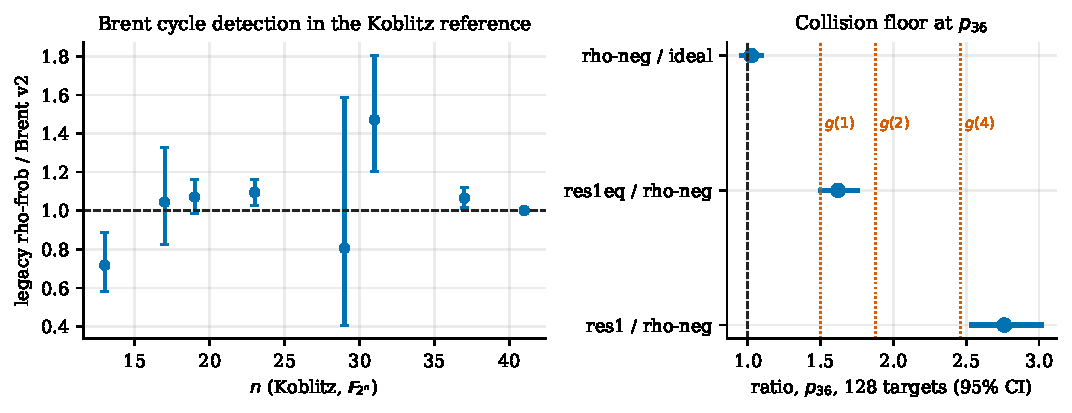
\includegraphics[width=\linewidth]{figures/fig-nov-reference.pdf}
\caption[]{Left: legacy Koblitz rho over Brent v2, fully priced, 95\%
intervals (32 targets $\times$ 3 rounds per curve). Right: at $p_{36}$, rho-neg
against its ideal, and the residual collectors against rho-neg, with the
collision floors $g(k)$. Sources:
\art{research/rho_frob_brent_20261106/README.md},
\art{research/ic_rho_floor_20261109/README.md}.}
\label{fig:nov-reference}
\end{figure}

\paragraph{Instruction audits.} The hyperelliptic ecbench row passes. Its
IC and rho arms run $1{,}259$ and $1{,}313$ instructions per kilo-gate, so
its IC/rho of $0.207$ is a ratio of audited counts
(\art{research/ic_acct3_hec_ecbench_20261021/AUDIT_IR.md}). The weak-class
cover row (IC/rho $0.0098$ $[0.0069,0.0144]$) is \emph{not admitted}, for
two reasons (\art{research/ic_acct1_cover_bitop_20261021/AUDIT_IR.md}):
\begin{itemize}
\item its IC arm spends $18\times$ rho's instructions per counted gate, and
  still $8.1\times$ with the counting hooks idle;
\item its committed IC rows reproduce at the study commit but not at
  \texttt{main} ($-13.0\%$ and $-8.7\%$ totals).
\end{itemize}

\section{$k=4$ in characteristic two reaches $m=18$}\label{sec:nov-k4}

Chapter~\ref{ch:extension} recorded the ladder through $m=17$ and no
record at $m=18$. The study's README now carries an $m=18$ IC record
(\art{research/gaudry_k4_char2_crossover_20261015/README.md}). Against rho's
theoretical $0.886\sqrt r$, the geometric means of IC over rho are $3.64$,
$1.68$, $0.95$ and $0.45$ at $m=15$--$18$. The fitted slope is $-0.246$
against the expected $-1/4$, and the interpolated crossing is
$m^\ast\approx16.9$ ($\log_2 n^\ast\approx67.7$). The study states the limits
itself:
\begin{itemize}
\item two targets per size at $m=15$--$17$, and one at $m=18$, whose rho run
  was still running;
\item measured-against-measured IC/rho scatters from $0.62$ to $19$ at one
  size;
\item no session has been replayed, and the completed runs used a
  checkpointing binary whose source is not on \texttt{main}.
\end{itemize}
The relayed red-team review projects $m^\ast\approx17.6$ ($16.3$--$19.2$)
and calls the crossover \emph{not established}. The Wiedemann matrix grows to
2.57\% of IC cost at $m=18$, and large primes lose at every reachable size.
This remains a weak family and the cheapest place a measured crossover could
go on record (Chapter~\ref{ch:conclusion}, item~3).

\begin{figure}[t]
\centering
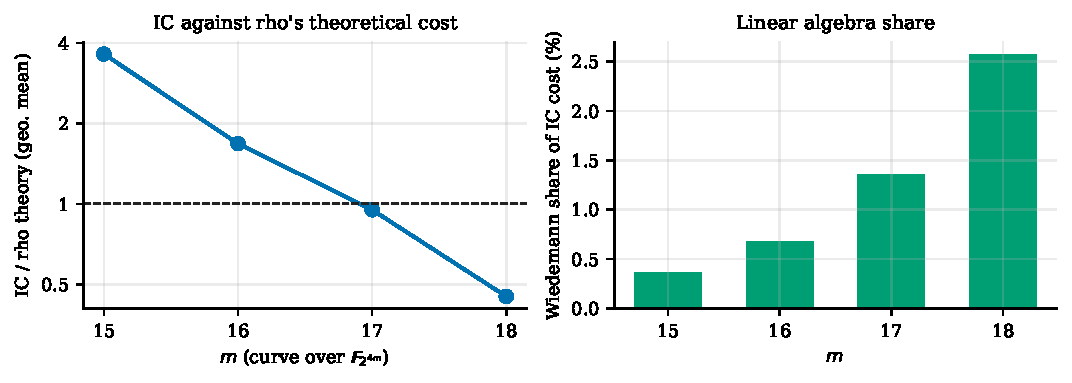
\includegraphics[width=\linewidth]{figures/fig-nov-k4.pdf}
\caption[]{$k=4$ over $\FF_{2^{4m}}$, $h=2$: IC over rho's theoretical cost
(geometric mean per size; $m=18$ is one target), and the sparse
linear-algebra share of IC cost. Single targets, not replayed. Source:
\art{research/gaudry_k4_char2_crossover_20261015/README.md}.}
\label{fig:nov-k4}
\end{figure}

\section{Prime fields: no lever}\label{sec:nov-prime}

\paragraph{Minors guess-and-determine: closed}
(\art{research/minors_guess_determine_20261107/RESULTS.md}). The cheapest arm
costs $4.37$ $[4.28,4.46]\times$ matched rho at 20 bits and $1552$
$[1049,2721]\times$ at 40 bits. Its exponent exceeds rho's by $0.42$--$0.47$
over all sizes.

\paragraph{PKM fall degree: tracks the presentation}
(\art{research/pkm_falldegree_unblock_20261107/RESULTS.md},
\art{research/pkm_matched_prime_20261106/README.md}). Stage~A (Kummer,
$m=2$, prime $P_1$) repeats the session-reported values of
\S\ref{sec:fd-pkm} at $t\le10$ and extends them: the median $d_F$ is
$3,4,4,4,4,5,5,5,5,6,6$ at $t=1$--$11$. The random-coefficient null arm is
identical. On matched primes the degree follows $t$, not $p$. Two parts did
not finish:
\begin{itemize}
\item the C-step prediction holds at $t=11,12$ and is undecided at
  $t=13,14$;
\item stage~B was lost to Spot interruptions.
\end{itemize}
This is the first committed raw data for the Kummer last fall degrees that
Appendix~\ref{app:artefacts} lists as session-reported.

\begin{figure}[t]
\centering
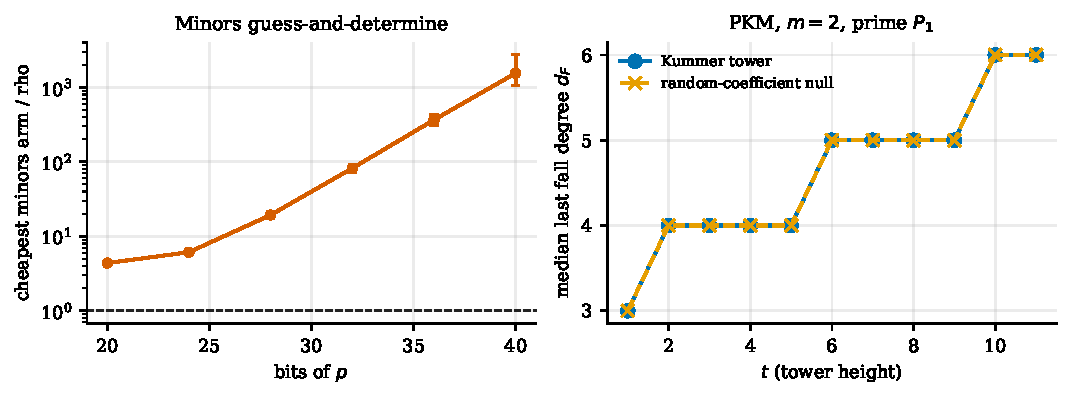
\includegraphics[width=\linewidth]{figures/fig-nov-prime.pdf}
\caption[]{Left: cheapest minors guess-and-determine arm over matched rho
(95\% intervals). Right: median last fall degree of PKM Kummer towers,
$m=2$, prime $P_1$, tower and random-coefficient null (identical). Sources:
\art{research/minors_guess_determine_20261107/RESULTS.md},
\art{research/pkm_falldegree_unblock_20261107/RESULTS.md}.}
\label{fig:nov-prime}
\end{figure}

\paragraph{Other closures.}
\begin{itemize}
\item \emph{\texttt{ic\_e222\_m221} campaign.} The single-target IC walk costs
  at least $25$--$53\times$ matched negation rho at 20--24 bits
  (\art{research/ic_e222_m221_20261106/CAMPAIGN_SUMMARY.md}).
\item \emph{Split-graph secant presentation.} Rejected at the tested scale for
  both candidates, and unranked under \S5a
  (\art{research/split_graph_secant_cost_20261107/RESULTS.md}).
\item \emph{Small coefficients in the ECCp-131 isogeny class.} Flat for
  $S_3$ yield: $0.987$ $[0.928,1.051]$ at $p\approx2^{40.3}$. Reaching a
  small-coefficient member takes about $2^{67.6}$ candidates, against
  rho's $2^{64.9}$ (\art{research/coeff_model_semaev_20261109/report/REPORT.md}).
\item \emph{Trace-zero factor base.} The coverage deficit is $0.003$, far
  below usable (\art{research/tracezero_toy_20261106/README.md}).
\item \emph{Split primes.} The pattern reaches $E(\FF_p)$ only through known
  scalars (\art{research/split_prime_ecdlp_20261107/}).
\item \emph{Lead assessment.} The 7 November assessment finds no open
  prime-field lead with a credible exponent mechanism
  (\art{research/prime_field_lead_assessment_20261107/README.md}).
\end{itemize}
The 10 November sweep ran 173 leads once each at toy scale under one frozen
protocol. It recorded 98 consistent, 28 falsified, 42 inconclusive and 5
not run, and found no evidence of a below-$\sqrt p$ exponent. Its two
``possible signal'' flags are read as pre-asymptotic artefacts
(\art{research/lead_sweep_20261110/SWEEP_REPORT.md}).

\section{Binary engines and factor bases}\label{sec:nov-binary}

\begin{itemize}
\item \emph{M4GB} (\art{research/m4gb_integration_20261110/RESULTS.md},
  \art{research/m4gb_descent_ladder_20261110/README.md}). The kernel patch
  speeds GF(31) up $3.4$--$4.1\times$ and leaves GF(2) unchanged. On the
  descent ladder, M4GB overtakes the in-house full-basis \texttt{f4-f2}
  from about 22 unknowns: 489\,ms against 2{,}059\,ms at 24 unknowns.
  \texttt{inherited-f4} is still $10$--$90\times$ faster on every cell, so
  it remains the decomposition oracle.
\item \emph{Prefix-cached F4 root.} Exact, but a null: $0.989$--$1.006\times$
  (\art{research/f4_prefix_root_20261109/README.md}).
\item \emph{Guess-and-determine degree.} Five guesses hold degree~4 at
  $\ell=9$ on 3 of 4 draws, against the 7 that the registered model
  predicted (\art{research/dreg_guess_scaling_20261106/RESULTS.md}). The
  kind of guess made no detectable difference.
\item \emph{Frobenius pair tables.} Build-time collisions give no free
  relations: rank 0 on all 8 cells, because every collision is a symmetry
  (\art{research/frobenius_table_free_rows_20261106/README.md}).
\item \emph{Conjugate-pair lines over $\FF_{q^4}$}
  (\art{research/lift_dense_conjugate_pair_cost_20261106/README.md},
  \art{research/lift_dense_conjugate_pair_infinity_20261106/README.md}).
  On curves with full 2-torsion they give about $36\times$ the relations per
  trial of the standard line ($36.6$ at $q=13$, $35.8$ at $q=101$), with
  $11$--$17\times$ fewer trials to full rank, at equal per-trial solve cost.
  Solver failures were 3-point decompositions at infinity; a random chart
  recovers 19 of 20. This is IC-versus-IC at toy scale. It needs a cofactor
  divisible by 4 and never applies to prime-order curves.
\item \emph{Joux--Vitse weighted grading.} About $670\times$ dearer than the
  current solver at $p=271$
  (\art{research/jv_weighted_grading_20261106/README.md}).
\end{itemize}

\section{Unconventional routes}\label{sec:nov-exotic}

\begin{itemize}
\item \emph{Hashed tensor ECDL.} The reduction is correct, but the route is
  at least 120 bits above rho at $b=128$--$256$, even at the impossible
  $a=1$ (\art{research/hashed_ecdl_tensor_audit_20261107/README.md}).
\item \emph{ML learnability control.} 0 signal, 22 null and 2 underpowered
  cells (\art{research/ml_learnability_control_20261107/RESULTS.md}; the
  directory's README predates its results).
\item \emph{Elliptic-code list decoding.} Unresolved by its frozen rule: the
  decoder is never cheaper than enumeration
  (\art{research/elliptic_code_list_decoding_20261107/RESULTS.md}).
\item \emph{Literature sweep.} 1{,}601 items, and no cost-model number changes
  (\art{research/lit_sweep_20261107/README.md}).
\end{itemize}

\section{What did not run}\label{sec:nov-blocked}

The following studies hold no data yet:
\begin{itemize}
\item \art{research/c1_end_to_end_solve_20261107/} and
  \art{research/arity_completion_20261104/}: protocols frozen, not run;
\item \art{research/m4gb_e2e_ic_ladder_20261110/}: results not summarised;
\item \art{research/gpu_ic_baseline_20261027/}: design only;
\item \art{research/ecdl_tensor_ic_cofactor_speed_20261107/}: frozen, not run;
\item \art{research/fall_degree_bounds_20261008/}: runs E13 and E14 did
  not complete.
\end{itemize}
The last of these is the item that bears most on Chapter~\ref{ch:falldegree}.
Certifying more instances at $n=33$--$51$ is still the open step.

\paragraph{Net effect.} Nothing in the window moves an exponent, and the
summary of Chapter~\ref{ch:distance} stands.
\begin{itemize}
\item The changes to the reference make rho stronger or leave it unchanged
  (table pricing, Brent where adopted, the hyperelliptic default walk), or
  correct how a prime gap is normalised (medium tier).
\item The closest approach to rho on a prime-order curve is a boundary
  method, $1.22$--$1.40\times$, that is not index calculus.
\end{itemize}
